\section{Introduction to mk-query-digest}

\begin{frame}
   \frametitle{What is mk-query-digest?}
   \begin{block}{General-purpose ``query event processor''}
      \begin{itemize}
         \item Extract \emph{query events} from some input
         \item Pass the events through a \emph{pipeline}
         \item Apply transformations, filtering, aggregation\dots
         \item Perform many different types of actions with the events
         \item Produce some output when done
      \end{itemize}
   \end{block}
   
\includegraphics[width=20mm]{../image/wizard}
\end{frame}

\begin{frame}
   \frametitle{Query Events}
   \begin{block}{A data structure that represents an occurrence of a query}
      \begin{itemize}
         \item Internally, it's a Perl hash table
         \item It's just a key-value data structure
         \item In Maatkit-world, we refer to the data as \emph{attributes}
      \end{itemize}
   \end{block}
   \begin{block}{Common query event attributes}
      \begin{center}
      \begin{tabular}{ll}
         Attribute Name & Meaning \\
         \hline
         arg         & The text of the query \\
         cmd         & The type of the event \\
         ts          & The timestamp of the event \\
         db          & Database \\
         Query\_time & Execution time / response time \\
         pos\_in\_log & The event's byte offset in the input \\
      \end{tabular}
      \end{center}
   \end{block}
\end{frame}

\begin{frame}
   \frametitle{The event pipeline}
   \begin{block}{How the pipeline works}
   \begin{enumerate}
      \item Get events from the source
      \item Pre-filter (for options such as \texttt{--since} and \texttt{--until})
      \item Apply some default transformations, such as adding a \emph{fingerprint} to the event
      \item Apply user-defined filters/functions to the events
      \item Special-purpose filters: execute the event against a database, add a delay into the pipeline, do a ``query review''\dots
      \item Aggregate events together
      \item Compute and display a report
   \end{enumerate}
   \end{block}

   
\includegraphics[width=15mm]{../image/magnify}
   
\includegraphics[width=5mm]{../image/next}
   
\includegraphics[width=15mm]{../image/filter}
   
\includegraphics[width=5mm]{../image/next}
   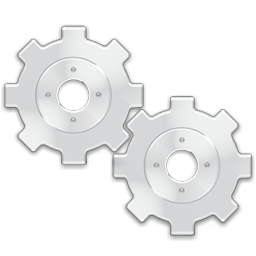
\includegraphics[width=15mm]{../image/exec}
   
\includegraphics[width=5mm]{../image/next}
   
\includegraphics[width=15mm]{../image/funct}
   
\includegraphics[width=5mm]{../image/next}
   
\includegraphics[width=15mm]{../image/aggregate}
   
\includegraphics[width=5mm]{../image/next}
   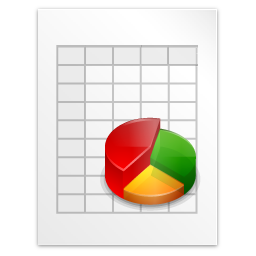
\includegraphics[width=15mm]{../image/spreadsheet_document}

\end{frame}

\begin{frame}[fragile]
   \frametitle{Fingerprints}
   \begin{block}{What is a fingerprint?}
   \begin{itemize}
      \item A fingerprint is a normalized/abstracted form of a query
      \item Whitespace collapsed, comments removed, literals replaced by \texttt{?}
      \item Many other transformations are applied (collapsing IN lists\dots)
      \item Example:
\begin{verbatim}
SELECT *
  FROM   users
 WHERE   id IN('eeyore','pooh'); -- where's piglet?
\end{verbatim}
      \item Result:
\begin{verbatim}
select * from users where id in(?);
\end{verbatim}
   \end{itemize}
   \end{block}
   
\includegraphics[width=20mm]{../image/fingerprint}
\end{frame}

\begin{frame}
   \frametitle{The default report}
   \begin{enumerate}
      \item Fingerprint every event
      \item Auto-detect attributes, and run stats on numeric attributes
      \item Aggregate events by fingerprint; place them into classes
      \item Sort the classes by total Query\_time
      \item Keep the ``short head'' and queries that perform very badly
      \item Print out a report on each noteworthy class of queries
   \end{enumerate}
\end{frame}

\begin{frame}[fragile]
   \frametitle{Demo: the default report}

   If you want to follow along, try this:

   \scriptsize

\begin{verbatim}
wget http://www.maatkit.org/get/mk-query-digest
wget http://maatkit.googlecode.com/svn/trunk/common/t/samples/pg-sample2
perl mk-query-digest --type pglog pg-sample2
\end{verbatim}

   \normalsize

   
\includegraphics[width=20mm]{../image/demo}
\end{frame}

\begin{frame}[fragile]
\frametitle{Default report header}
\begin{block}{Info about the whole report}
\begin{itemize}
   \item This file has 884 query events, and 69 different fingerprints
   \item There's a table of stats for the numeric attributes
\end{itemize}
\end{block}
\scriptsize
\begin{verbatim}
# 860ms user time, 50ms system time, 14.89M rss, 20.06M vsz
# Overall: 884 total, 69 unique, 0 QPS, 0x concurrency ___________________
#                    total     min     max     avg     95%  stddev  median
# Exec time             3s   147us    72ms     3ms    10ms     8ms     1ms
# bytes            170.18k      39     569  197.14  563.87  186.59   92.72
\end{verbatim}
\normalsize
\end{frame}

\begin{frame}[fragile]
\frametitle{Default report for one fingerprint}
\begin{block}{A report on a single fingerprint's queries}
\end{block}
\scriptsize
\begin{verbatim}
# Query 1: 0 QPS, 0x concurrency, ID 0x8FFEBD609B778EB2 at byte 97807 ____
# This item is included in the report because it matches --limit.
#              pct   total     min     max     avg     95%  stddev  median
# Count          7      67
# Exec time     22   631ms     4ms    72ms     9ms    14ms     8ms     8ms
# bytes          6  11.73k     155     335  179.31  202.40   31.22  166.51
# Query_time distribution
#   1us
#  10us
# 100us
#   1ms  ################################################################
#  10ms  #############################
# 100ms
#    1s
#  10s+
# Tables
#    SHOW TABLE STATUS LIKE 'activity_log'\G
#    SHOW CREATE TABLE `activity_log`\G
INSERT INTO activity_log <.... rest of query ....>
\end{verbatim}
\normalsize
\end{frame}

\begin{frame}[fragile]
\frametitle{Default report profile}
\begin{block}{A profile of the queries, sorted by \emph{R} descending}
\end{block}
\scriptsize
\begin{verbatim}
# Profile
# Rank Query ID           Response time    Calls R/Call   Item
# ==== ================== ================ ===== ======== ===============
#    1 0x8FFEBD609B778EB2     0.6307 25.2%    67   0.0094 INSERT activity
#    2 0x1C55D6804083DB4C     0.3908 15.6%     7   0.0558 SELECT stats_cv
#    3 0x62EC2BC35CD62D85     0.3519 14.1%     7   0.0503 SELECT stats_cv
#    4 0x32AF9886FDBBAE30     0.1513  6.0%   144   0.0011 SELECT frs_file
#    5 0x1929E67B76DC55E7     0.1330  5.3%     3   0.0443 SELECT frs_dlst
#    6 0x60D6962E42C08882     0.1204  4.8%    67   0.0018 SELECT plugins
#    7 0xF2AF6DF05892D03E     0.1128  4.5%     5   0.0226 SELECT doc_data
#    8 0x64F8E6F000640AF8     0.0672  2.7%     3   0.0224 SELECT users
#    9 0x4636BFC0875521C9     0.0664  2.7%    93   0.0007 SELECT supporte
#   10 0x02CC64324ED7CA2C     0.0651  2.6%    12   0.0054 INSERT frs_dlst
\end{verbatim}
\normalsize
\end{frame}

\begin{frame}
   \frametitle{Sources of input}
   \begin{block}{mk-query-digest understands many types of input}
   \begin{center}
   \begin{tabular}{ll}
   Argument to \texttt{--type}
      \footnote{You can also use the \texttt{--processlist} option to get queries from MySQL's SHOW FULL PROCESSLIST}
   & Meaning \\
   \hline
   slowlog (default) & MySQL's ``slow query log'' \\
   binlog & Output of MySQL's mysqlbinlog program \\
   genlog & MySQL's ``general log'' (log of all queries) \\
   http   & HTTP TCP/IP traffic from tcpdump \\
   pglog  & PostgreSQL logs (stdout or syslog) \\
   tcpdump & MySQL TCP/IP traffic from tcpdump \\
   memcached & memcached TCP/IP traffic from tcpdump \\
   \end{tabular}
   \end{center}
   \end{block}
\end{frame}

\begin{frame}
   \frametitle{Important and useful options}
   \begin{block}{mk-query-digest has 50+ command-line options!}
   \begin{itemize}
      \item \texttt{--filter}, \texttt{--since}, and \texttt{--until}
      \item \texttt{--explain}
      \item \texttt{--group-by} and \texttt{--order-by}
      \item \texttt{--print}
      \item \texttt{--review} and \texttt{--review-history}
   \end{itemize}
   \end{block}
\end{frame}

\begin{frame}
   \frametitle{The \texttt{--filter} option}
   \begin{itemize}
      \item You can write arbitrary Perl code to filter and transform events
      \item Be sure it returns a true value so the pipeline continues
      \item Example: \texttt{--filter '\$event->\{db\} eq "mydb"'}
      \item The documentation has more examples
      \item The \texttt{--until} and \texttt{--since} options are just filters
   \end{itemize}
   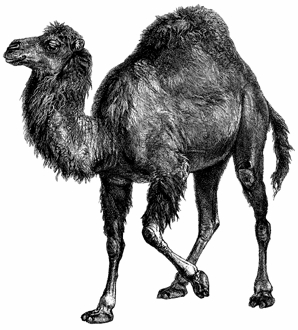
\includegraphics[width=20mm]{../image/perl}
\end{frame}

\begin{frame}
   \frametitle{The \texttt{--explain} option}
   \begin{itemize}
      \item You can get the database to EXPLAIN your queries
      \item See the results right in the report
   \end{itemize}
\end{frame}

\begin{frame}
   \frametitle{The \texttt{--group-by} option}
   \begin{itemize}
      \item Defines how queries are aggregated into classes
      \item Not quite like SQL's \texttt{GROUP BY}
      \item Default is \texttt{fingerprint}
      \item Special values: \texttt{distill}, \texttt{tables}
      \item Multiple reports: \texttt{--group-by fingerprint,tables,distill}
   \end{itemize}
\end{frame}

\begin{frame}
   \frametitle{The \texttt{--order-by} option}
   \begin{itemize}
      \item Defines what is ``worst'', and how to sort the report
      \item The sample query is ``worst in class'' by this criterion
      \item Default is \texttt{Query\_time:sum}
      \item You could also sort by other pseudo-attributes such as \texttt{:max}
   \end{itemize}
\end{frame}

\begin{frame}
   \frametitle{The \texttt{--print} option}
   \begin{itemize}
      \item Prints out events in MySQL's ``slow query log'' format
      \item Maatkit uses this format as its \emph{lingua franca}
      \item Other Maatkit tools can accept this input (example: mk-query-advisor)
      \item You probably want to use \texttt{--no-report} with this
   \end{itemize}
\end{frame}

\begin{frame}
   \frametitle{The \texttt{--review} option}
   \begin{itemize}
      \item Tired of reviewing the same queries every day?
      \item Store them into a table, with arbitrary meta-data
      \item See only ``new'' queries in the report!
      \item With \texttt{--review-history}, store report stats too
   \end{itemize}
   
\includegraphics[width=20mm]{../image/database_search}
\end{frame}
